
\documentclass[a4paper,10pt]{article}
\usepackage[top=2cm, left=2.5cm, right=2.5cm, bottom=2cm]{geometry}
\usepackage[cmex10]{amsmath}
\usepackage{graphicx}
\usepackage{gvv-book}
\usepackage{gvv}
\usepackage{textcomp}
\usepackage{multicol}

\begin{document}

\title{2024 - AR : Architecture and Planning Exam}
\author{Puni Aditya - EE25BTECH11046}
\date{16th August, 2025}
\maketitle
Duration: Three Hours \hfill Maximum Marks:100

\section*{General Aptitude (GA)}

\begin{enumerate}
    \item If '$\to$' denotes increasing order of intensity, then the meaning of the words [sick $\to$ infirm $\to$ moribund] is analogous to [silly $\to$ \rule{2cm}{0.4pt} $\to$ daft]. Which one of the given options is appropriate to fill the blank?
    \begin{multicols}{4}
    \begin{enumerate}
        \item frown
        \item fawn
        \item vein
        \item vain
    \end{enumerate}
    \end{multicols}
    \hfill (GATE-AR 2024)

    \item The 15 parts of the given figure are to be painted such that no two adjacent parts with shared boundaries (excluding corners) have the same color. The minimum number of colors required is
    \begin{figure}[h!]
    \centering
    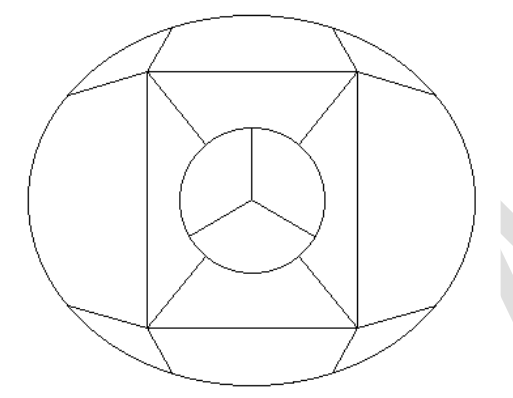
\includegraphics[width=0.5\columnwidth]{figs/01.jpg}
    \caption{}
    \label{fig:Img01}
    \end{figure}
    \begin{multicols}{4}
    \begin{enumerate}
        \item 4
        \item 3
        \item 5
        \item 6
    \end{enumerate}
    \end{multicols}
    \hfill (GATE-AR 2024)

    \item How many 4-digit positive integers divisible by 3 can be formed using only the digits \cbrak{1, 3, 4, 6, 7}, such that no digit appears more than once in a number?
    \begin{multicols}{4}
    \begin{enumerate}
        \item 24
        \item 48
        \item 72
        \item 12
    \end{enumerate}
    \end{multicols}
    \hfill (GATE-AR 2024)

    \item The sum of the following infinite series is
    $2 + \frac{1}{2} + \frac{1}{3} + \frac{1}{4} + \frac{1}{8} + \frac{1}{9} + \frac{1}{16} + \frac{1}{27} + \cdots$
    \begin{multicols}{4}
    \begin{enumerate}
        \item $\frac{11}{3}$
        \item $\frac{7}{2}$
        \item $\frac{13}{4}$
        \item $\frac{9}{2}$
    \end{enumerate}
    \end{multicols}
    \hfill (GATE-AR 2024)

    \item In an election, the share of valid votes received by the four candidates A, B, C, and D is represented by the pie chart shown. The total number of votes cast in the election were 1,15,000, out of which 5,000 were invalid. Based on the data provided, the total number of valid votes received by the candidates B and C is
    \begin{figure}[h!]
    \centering
    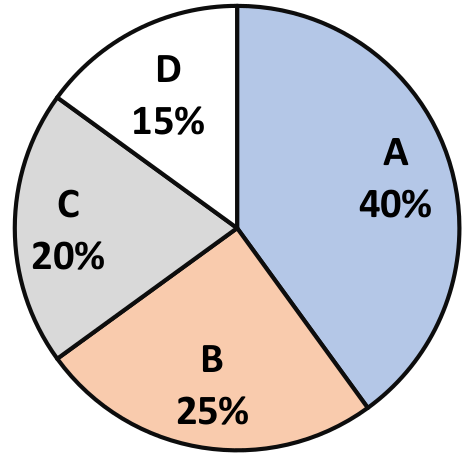
\includegraphics[width=0.5\columnwidth]{figs/02.jpg}
    \caption{Share of Valid Votes}
    \label{fig:Img02}
    \end{figure}
    \begin{multicols}{4}
    \begin{enumerate}
        \item 45,000
        \item 49,500
        \item 51,750
        \item 54,000
    \end{enumerate}
    \end{multicols}
    \hfill (GATE-AR 2024)

    \item Thousands of years ago, some people began dairy farming. This coincided with a number of mutations in a particular gene that resulted in these people developing the ability to digest dairy milk. Based on the given passage, which of the following can be inferred?
    \begin{enumerate}
        \item All human beings can digest dairy milk.
        \item No human being can digest dairy milk.
        \item Digestion of dairy milk is essential for human beings.
        \item In human beings, digestion of dairy milk resulted from a mutated gene.
    \end{enumerate}
    \hfill (GATE-AR 2024)

    \item The probability of a boy or a girl being born is $\frac{1}{2}$. For a family having only three children, what is the probability of having two girls and one boy?
    \begin{multicols}{4}
    \begin{enumerate}
        \item $\frac{3}{8}$
        \item $\frac{1}{8}$
        \item $\frac{1}{4}$
        \item $\frac{1}{2}$
    \end{enumerate}
    \end{multicols}
    \hfill (GATE-AR 2024)

    \item Person 1 and Person 2 invest in three mutual funds A, B, and C. The amounts they invest in each of these mutual funds are given in the table. \\
    \begin{tabular}{ | c | c | c | c | }
    \hline
    & Mutual fund A & Mutual fund B & Mutual fund C \\
    \hline
    Person 1 & Rs.10,000 & Rs.20,000 & Rs.20,000 \\
    \hline
    Person 2 & Rs.20,000 & Rs.15,000 & Rs.15,000 \\
    \hline
    \end{tabular} \\
    At the end of one year, the total amount that Person 1 gets is Rs.500 more than Person 2. The annual rate of return for the mutual funds B and C is 15\% each. What is the annual rate of return for the mutual fund A?
    \begin{multicols}{4}
    \begin{enumerate}
        \item 7.5\%
        \item 10\%
        \item 15\%
        \item 20\%
    \end{enumerate}
    \end{multicols}
    \hfill (GATE-AR 2024)

\newpage

    \item Three different views of a dice are shown in the figure below. \\
    \begin{figure}[h!]
    \centering
    
\includegraphics[width=0.2\columnwidth]{figs/03.jpg}
    \caption{Dice}
    \label{fig:Img03}
    \end{figure}
    The piece of paper that can be folded to make this dice is
    \begin{enumerate}
        \item \begin{figure}[h!]
    \centering
    
\includegraphics[width=0.12\columnwidth]{figs/04.jpg}
    \caption{}
    \label{fig:Img04}
    \end{figure}
        \item \begin{figure}[h!]
    \centering
    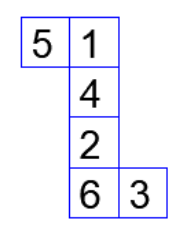
\includegraphics[width=0.12\columnwidth]{figs/05.jpg}
    \caption{}
    \label{fig:Img05}
    \end{figure}
        \item \begin{figure}[h!]
    \centering
    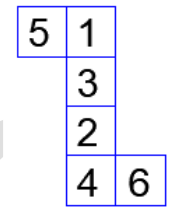
\includegraphics[width=0.12\columnwidth]{figs/06.jpg}
    \caption{}
    \label{fig:Img06}
    \end{figure}
        \item \begin{figure}[h!]
    \centering
    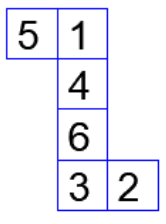
\includegraphics[width=0.12\columnwidth]{figs/07.jpg}
    \caption{}
    \label{fig:Img07}
    \end{figure}
    \end{enumerate}
    \hfill (GATE-AR 2024)
    
    \item Visualize two identical right circular cones such that one is inverted over the other and they share a common circular base. If a cutting plane passes through the vertices of the assembled cones, what shape does the outer boundary of the resulting cross-section make?
    \begin{multicols}{4}
    \begin{enumerate}
        \item A rhombus
        \item A triangle
        \item An ellipse
        \item A hexagon
    \end{enumerate}
    \end{multicols}
    \hfill (GATE-AR 2024)

\section*{PART A: Common FOR ALL CANDIDATES}

    \item The nature of curvature of the following structural form is
    \begin{figure}[h!]
    \centering
    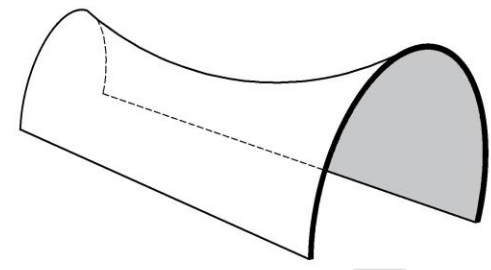
\includegraphics[width=0.5\columnwidth]{figs/08.jpg}
    \caption{}
    \label{fig:Img08}
    \end{figure}
    \begin{multicols}{4}
    \begin{enumerate}
        \item monoclastic
        \item synclastic
        \item anticlastic
        \item mobius
    \end{enumerate}
    \end{multicols}
    \hfill (GATE-AR 2024)

    \item As per the Ekistics Logarithmic Scale, the 'world city' is referred as
    \begin{multicols}{4}
    \begin{enumerate}
        \item Megalopolis
        \item Conurbation
        \item Acropolis
        \item Ecumenopolis
    \end{enumerate}
    \end{multicols}
    \hfill (GATE-AR 2024)

    \item In Manasara Silpasastra, a bow-shaped town plan is known as
    \begin{multicols}{4}
    \begin{enumerate}
        \item Dandaka
        \item Prastara
        \item Karmuka
        \item Nandyavarta
    \end{enumerate}
    \end{multicols}
    \hfill (GATE-AR 2024)

    \item The value of a property when sold at a lower price than its open market price is called
    \begin{multicols}{2}
    \begin{enumerate}
        \item Distress Value
        \item Accommodation Value
        \item Speculative Value
        \item Replacement Value
    \end{enumerate}
    \end{multicols}
    \hfill (GATE-AR 2024)

    \item In a traffic survey, Enoscope is used to measure
    \begin{multicols}{4}
    \begin{enumerate}
        \item Volume to Capacity ratio
        \item Sight distance
        \item Spot speed
        \item Intersection delay
    \end{enumerate}
    \end{multicols}
    \hfill (GATE-AR 2024)

    \item The author of the book Human Aspects of Urban Form is
    \begin{multicols}{4}
    \begin{enumerate}
        \item Cliff Moughtin
        \item Amos Rapoport
        \item Peter Katz
        \item Lewis Mumford
    \end{enumerate}
    \end{multicols}
    \hfill (GATE-AR 2024)

    \item Which of the following statements is correct for Urban Cool Island (UCI)?
    \begin{enumerate}
        \item The UCI and Urban Heat Island (UHI) cannot happen in a city at the same time.
        \item Air temperature of surrounding rural areas is warmer than that of the urban areas.
        \item Air temperature of surrounding rural areas is cooler than that of the urban areas.
        \item UCI happens only in a snow-clad mountain.
    \end{enumerate}
    \hfill (GATE-AR 2024)

    \item Which of the following statements is correct for an oxidation pond to treat waste water?
    \begin{enumerate}
        \item It is an aerobic pond.
        \item It is an anaerobic pond.
        \item It does not require sunlight.
        \item It does not remove Biological Oxygen Demand (BOD).
    \end{enumerate}
    \hfill (GATE-AR 2024)

    \item The conservation architect of the Maitreya Buddha Temple at Basgo, Ladakh which won the 2007 UNESCO Asia-Pacific Heritage Award is
    \begin{multicols}{2}
    \begin{enumerate}
        \item Abha Narain Lambah
        \item Vinod Kumar M. M.
        \item Rahul Mehrotra
        \item Saima Iqbal
    \end{enumerate}
    \end{multicols}
    \hfill (GATE-AR 2024)

    \item Which of the following options is/are the right sequence(s) in water treatment process?
    \begin{enumerate}
        \item Coagulation $\to$ Flocculation $\to$ Sedimentation
        \item Sedimentation $\to$ Filtration $\to$ Disinfection
        \item Sedimentation $\to$ Flocculation $\to$ Coagulation
        \item Disinfection $\to$ Filtration $\to$ Flocculation
    \end{enumerate}
    \hfill (GATE-AR 2024)

    \item Which of the following is/are associated with Gentrification in a neighbourhood?
    \begin{enumerate}
        \item Wealthier households displace poor households
        \item Poor households displace wealthier households
        \item Real estate value increases
        \item Real estate value decreases
    \end{enumerate}
    \hfill (GATE-AR 2024)

    \item Which of the following sites is/are included in the UNESCO World Heritage List as on December 2022?
    \begin{enumerate}
        \item Capitol Complex, Chandigarh
        \item Moth ki Masjid, Delhi
        \item Keoladeo National Park, Bharatpur
        \item Paradesi Synagogue, Kochi
    \end{enumerate}
    \hfill (GATE-AR 2024)

\newpage

    \item The reference points, lines and planes for drawing a two-point perspective of an object are marked in the Figure below. Select the correct option(s) that match(es) with the corresponding nomenclature.
    \begin{figure}[h!]
    \centering
    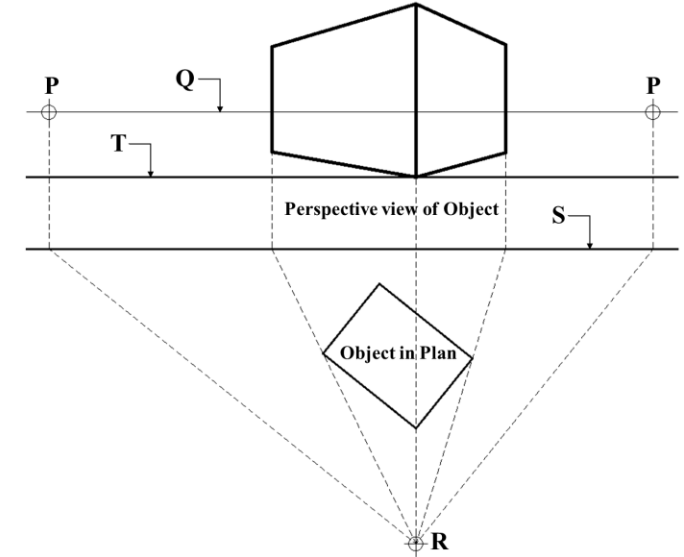
\includegraphics[width=0.5\columnwidth]{figs/09.jpg}
    \caption{}
    \label{fig:Img09}
    \end{figure}
    \begin{enumerate}
        \item R – Station point, S – Picture plane
        \item R – Vanishing point, T – Picture plane
        \item P – Vanishing point, T – Ground line
        \item Q – Ground line, S – Horizon line
    \end{enumerate}
    \hfill (GATE-AR 2024)

    \item India's intended Nationally Determined Contribution to the United Nations Framework Convention on Climate Change in 2022 include(s)
    \begin{enumerate}
        \item reduction of emissions intensity of India's GDP by 45\% by 2030 from 2005 level
        \item achieving about 50\% cumulative electric power installed capacity from non-fossil fuel-based energy resources by 2030
        \item achieving the target of net-zero emission by 2030
        \item reduction of total projected carbon emission by one billion tonnes from 2022 to 2025
    \end{enumerate}
    \hfill (GATE-AR 2024)

    \item As per the Census of India 2011, non-notified slums is/are categorised as
    \begin{multicols}{4}
    \begin{enumerate}
        \item Recognised
        \item Identified
        \item Unrecognised
        \item Authorised
    \end{enumerate}
    \end{multicols}
    \hfill (GATE-AR 2024)

    \item Which of the following is/are under the purview of the Energy Conservation Building Code of India 2017?
    \begin{multicols}{2}
    \begin{enumerate}
        \item Indoor Lighting
        \item Outdoor Lighting
        \item Plug Loads
        \item Embodied Energy
    \end{enumerate}
    \end{multicols}
    \hfill (GATE-AR 2024)

    \item Which of the following is/are used for municipal fiscal resource mobilisation?
    \begin{multicols}{2}
    \begin{enumerate}
        \item Property tax
        \item Development charges
        \item Income tax
        \item Salary of municipal staff
    \end{enumerate}
    \end{multicols}
    \hfill (GATE-AR 2024)

    \item A ramp with a slope of 1:12 is required for wheelchair access. Intermediate landings of length 1.5 m each have to be provided after every 9 m running length. The running length of a straight ramp including landing, to negotiate a level difference of 900 mm vertical height, in m, is \rule{2cm}{0.4pt} (rounded off to two decimal places). \\
    \hfill (GATE-AR 2024)

    \item Match the features in \textbf{Group—I} with the corresponding software tools in \textbf{Group—II}. \\
    \begin{tabular}{ l l }
    \textbf{Group—I} & \textbf{Group—II} \\
    (P) Raster Graphics Editing & (1) OpenStudio \\
    (Q) Energy Modeling & (2) GIMP \\
    (R) Visual Programming Interface & (3) STAAD \\
    (S) Structural Analysis & (4) Grasshopper \\
    & (5) Radiance \\
    \end{tabular}
    \begin{multicols}{2}
    \begin{enumerate}
        \item P—3, Q—1, R—2, S—5
        \item P—2, Q—1, R—4, S—3
        \item P—1, Q—4, R—5, S—2
        \item P—2, Q—5, R—1, S—3
    \end{enumerate}
    \end{multicols}
    \hfill (GATE-AR 2024)

    \item Match the elements in \textbf{Group—I} with the corresponding buildings in \textbf{Group—II}. \\
    \begin{tabular}{ l l }
    \textbf{Group—I} & \textbf{Group—II} \\
    (P) Lightweight Structure & (1) Taipei 101, Taipei by Lee and Wang \\
    (Q) Base Isolator & (2) The Gherkin, London by Foster \& Partners \\
    (R) Tuned-mass Damper & (3) Museum of New Zealand Te Papa \\
    & Tongarewa, Wellington by Ivan Mercep \\
    (S) Diagrid & (4) Paper Log Houses, Kobe by Shigeru Ban \\
    & (5) Metropolitan Cathedral of Christ the King, \\
    & Liverpool by Lutyens and Gibberd \\
    \end{tabular}
    \begin{multicols}{2}
    \begin{enumerate}
        \item P—1, Q—3, R—5, S—4
        \item P—4, Q—3, R—1, S—2
        \item P—4, Q—1, R—5, S—2
        \item P—3, Q—2, R—1, S—5
    \end{enumerate}
    \end{multicols}
    \hfill (GATE-AR 2024)

    \item Match the following concepts in \textbf{Group—I} with their corresponding description in \textbf{Group—II}. \\
    \begin{tabular}{ l l }
    \textbf{Group—I} & \textbf{Group—II} \\
    (P) N I M B Y & (1) Affording a clear view of the waterfront \\
    & to a plot through the abutting street \\
    (Q) Form based code & (2) Planning and zoning tool to regulate \\
    & development primarily through urban form \\
    (R) Tactical urbanism & (3) Establishment of residential areas on \\
    & the outskirts of a city \\
    (S) Suburbanisation & (4) Short-term, low cost, scalable interventions \\
    & and policies to change a neighbourhood \\
    & (5) Resisting any physical intervention by \\
    & public or private enterprises within \\
    & their neighbourhood \\
    \end{tabular}
    \begin{multicols}{2}
    \begin{enumerate}
        \item P—5, Q—2, R—4, S—3
        \item P—5, Q—4, R—3, S—2
        \item P—1, Q—2, R—4, S—5
        \item P—1, Q—5, R—4, S—3
    \end{enumerate}
    \end{multicols}
    \hfill (GATE-AR 2024)

    \item Match the urban renewal projects in \textbf{Group—I} with the corresponding cities in \textbf{Group—II}. \\
    \begin{tabular}{ l l }
    \textbf{Group—I} & \textbf{Group—II} \\
    (P) Cheonggyecheon & (1) New York \\
    (Q) The High Line & (2) London \\
    (R) False Creek South & (3) Seoul \\
    (S) Canary Wharf & (4) Vancouver \\
    & (5) Tokyo \\
    \end{tabular}
    \begin{multicols}{2}
    \begin{enumerate}
        \item P—3, Q—1, R—4, S—2
        \item P—3, Q—5, R—1, S—2
        \item P—5, Q—1, R—2, S—3
        \item P—2, Q—5, R—4, S—3
    \end{enumerate}
    \end{multicols}
    \hfill (GATE-AR 2024)

    \item Match the Biosphere Reserves in \textbf{Group—I} with their corresponding features in \textbf{Group—II}. \\
    \begin{tabular}{ l l }
    \textbf{Group—I} & \textbf{Group—II} \\
    (P) Gulf of Mannar & (1) Ridge, Glacier \\
    (Q) Sunderbans & (2) Sub-tropical/Tropical Forest, Stepped Hill \\
    (R) Nanda Devi & (3) Swamp forest, Mangrove \\
    (S) Nilgiri & (4) Coral Reefs, Seagrass bed \\
    & (5) Salt Marsh, Flat Terrain \\
    \end{tabular}
    \begin{multicols}{2}
    \begin{enumerate}
        \item P—1, Q—3, R—4, S—5
        \item P—3, Q—5, R—1, S—2
        \item P—4, Q—3, R—1, S—2
        \item P—4, Q—2, R—3, S—5
    \end{enumerate}
    \end{multicols}
    \hfill (GATE-AR 2024)

    \item Match the terminologies in \textbf{Group—I} with their descriptions in \textbf{Group—II}. \\
    \begin{tabular}{ l l }
    \textbf{Group—I} & \textbf{Group—II} \\
    (P) Edge City & (1) Rapid expansion of geographical areas \\
    & of towns or cities \\
    (Q) Synekism & (2) Violence against the city \\
    (R) Urbicide & (3) A secondary CBD on the edge of the city \\
    (S) Urban Sprawl & (4) Rebuilding core city area \\
    & (5) Union of several small urban settlements \\
    & under one rule \\
    \end{tabular}
    \begin{multicols}{2}
    \begin{enumerate}
        \item P—3, Q—5, R—2, S—1
        \item P—3, Q—4, R—2, S—5
        \item P—2, Q—5, R—3, S—1
        \item P—4, Q—2, R—3, S—1
    \end{enumerate}
    \end{multicols}
    \hfill (GATE-AR 2024)

    \item Match the items in \textbf{Group—I} with their corresponding items in \textbf{Group—II}. \\
    \begin{tabular}{ l l }
    \textbf{Group—I} & \textbf{Group—II} \\
    (P) Floating floor & (1) Overflow control \\
    (Q) Float valve & (2) Delay not affecting a project \\
    (R) Metal float & (3) Acoustical buffer \\
    (S) Free float & (4) Plastering equipment \\
    & (5) Traffic flow control \\
    \end{tabular}
    \begin{multicols}{4}
    \begin{enumerate}
        \item P—3, Q—2, R—4, S—1
        \item P—5, Q—1, R—3, S—4
        \item P—3, Q—1, R—4, S—2
        \item P—1, Q—2, R—5, S—4
    \end{enumerate}
    \end{multicols}
    \hfill (GATE-AR 2024)

    \item As per the URDPFI Guidelines 2015, match the type of educational facilities in \textbf{Group—I} with the corresponding minimum population to be served per facility in \textbf{Group—II}. \\
    \begin{tabular}{ l l }
    \textbf{Group—I} & \textbf{Group—II} \\
    (P) Integrated school & (1) 4,000 \\
    (Q) Senior secondary school & (2) 2,500 \\
    (R) College & (3) 90,000 \\
    (S) Primary school & (4) 1,25,000 \\
    & (5) 7,500 \\
    \end{tabular}
    \begin{multicols}{2}
    \begin{enumerate}
        \item P—4, Q—2, R—3, S—1
        \item P—3, Q—5, R—4, S—1
        \item P—2, Q—5, R—1, S—3
        \item P—3, Q—2, R—4, S—5
    \end{enumerate}
    \end{multicols}
    \hfill (GATE-AR 2024)

    \item Which of the following statements is/are true?
    \begin{enumerate}
        \item Physiological Equivalent Temperature is used in outdoor thermal comfort evaluation.
        \item Thermal Performance Index is computed using outside surface temperature of building envelope.
        \item Reynolds number less than 2000 refers to laminar wind flow.
        \item Reynolds number greater than 4000 refers to turbulent wind flow.
    \end{enumerate}
    \hfill (GATE-AR 2024)

    \item Which of the following statements is/are correct?
    \begin{enumerate}
        \item Yellow, blue-violet and red-violet are split complementary hues.
        \item Orange, green and violet are analogous combinations.
        \item CMYK is a subtractive colour system.
        \item Blue, green, orange and red are tetrad combinations.
    \end{enumerate}
    \hfill (GATE-AR 2024)

    \item Which of the following statements is/are correct?
    \begin{enumerate}
        \item The Royal Botanical Garden is in Kew, England.
        \item The Villa d'Este is in Tivoli, Italy.
        \item Indira Gandhi Memorial Tulip Garden is in Srinagar, J\&K, India.
        \item Shinjuku Gyoen National Garden is in Beijing, China.
    \end{enumerate}
    \hfill (GATE-AR 2024)

    \item Which of the following statements is/are correct?
    \begin{enumerate}
        \item Hibiscus or china rose (Hibiscus rosa-sinensis) is a shrub which has red, pink, white, and yellow blossoms.
        \item Frangipani, champa, and plumeria alba are names of the same flowering tree.
        \item Jacaranda (Jacarenda mimisifolia), gulmohar (delonix regia), and amaltas (laburnum) are flowering trees.
        \item The fruit of the Kadam/cadamba tree (Neolamarckia cadamba) is conical in shape and poisonous for humans.
    \end{enumerate}
    \hfill (GATE-AR 2024)

    \item Which of the following is/are component(s) of Right of Way (RoW) of a road?
    \begin{multicols}{4}
    \begin{enumerate}
        \item Building line
        \item Kerb
        \item Carriageway
        \item Sidewalk
    \end{enumerate}
    \end{multicols}
    \hfill (GATE-AR 2024)

    \item As per the National Building Code of India 2016, terminologies associated with fire fighting in a building is/are
    \begin{multicols}{2}
    \begin{enumerate}
        \item Refuge area
        \item Water sprinkler system
        \item Panic bar
        \item Atrium
    \end{enumerate}
    \end{multicols}
    \hfill (GATE-AR 2024)

\newpage

    \item For the beam shown below, ignoring the self-weight, the maximum hogging moment (in kN·m) generated for the loads indicated is \rule{2cm}{0.4pt} (rounded off to one decimal place). \\
    \begin{figure}[h!]
    \centering
    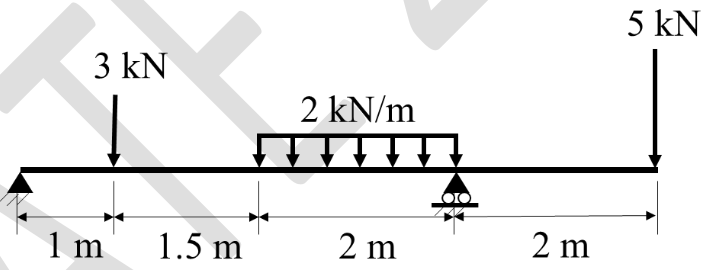
\includegraphics[width=0.5\columnwidth]{figs/10.jpg}
    \caption{Beam}
    \label{fig:Img10}
    \end{figure}
    \hfill (GATE-AR 2024)

    \item At present, the cost of a new office equipment is 50,000 (in Indian Rupees). It has 15\% salvage value after a useful life of 5 years. Using straight line method of depreciation, the book value of the equipment 3 years from now, in Indian Rupees, will be \rule{2cm}{0.4pt} (in integer). \\
    \hfill (GATE-AR 2024)

    \item The network diagram of a construction project is shown in the following Figure. The duration of each activity, in days, and the early start time of the project are denoted in the diagram. The total project duration along the critical path, in days, is \rule{2cm}{0.4pt} (in integer).
    \begin{figure}[h!]
    \centering
    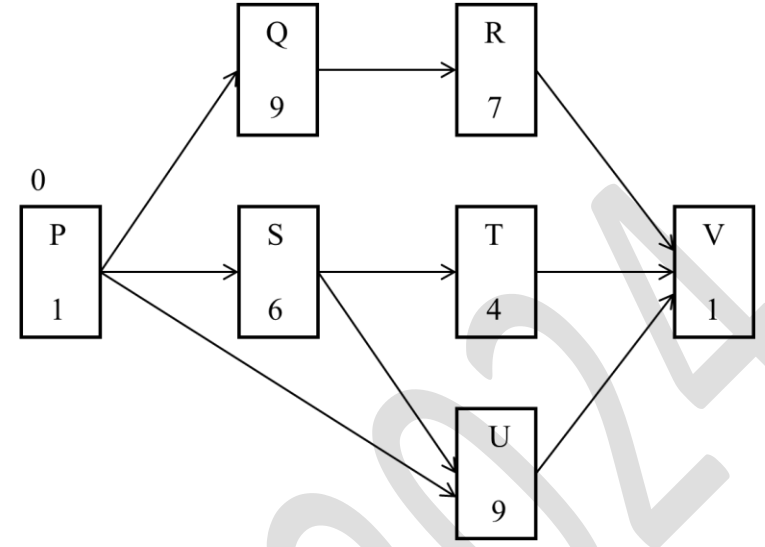
\includegraphics[width=0.5\columnwidth]{figs/11.jpg}
    \caption{}
    \label{fig:Img11}
    \end{figure}
    \hfill (GATE-AR 2024)

    \item The design of a 1200 capacity concert hall considers $\frac{1}{3}$\textsuperscript{rd} female audience and $\frac{2}{3}$\textsuperscript{rd} male audience. The Table below shows the guideline for calculating Water Closet requirements. \\
    \begin{tabular}{ | c | l | l | }
    \hline
    Fixture & Male & Female \\
    \hline
    Water closet & 1 number per 100 up to 400 and & 3 numbers per 100 up to 200 \\
    & over 400, 1 number for every & population and over 200, \\
    & 250 or part thereof & 2 numbers for every 100 or \\
    & & part thereof \\
    \hline
    \end{tabular} \\
    Using the above guideline, the number of Water Closets required for the total audience is \rule{2cm}{0.4pt} (in integer). \\
    \hfill (GATE-AR 2024)

    \item A declining Industrial Town has proposed to improve water sustainability by reducing stormwater runoff through change of land use land cover (LULC), as shown in the Table below, to attract new residents. \\
    \begin{tabular}{ | l | c | c | c | }
    \hline
    LULC & Runoff & Existing Area & Proposed Area \\
    & Coefficient & in hectare & in hectare \\
    \hline
    Industrial & 0.7 & 1500 & 800 \\
    \hline
    Residential & 0.5 & 1000 & 1200 \\
    \hline
    Park and Playgrounds & 0.25 & 1200 & 1000 \\
    \hline
    Forest & 0.15 & 300 & 1000 \\
    \hline
    \end{tabular} \\
    Considering a flat topography and zero additional runoff from the adjoining areas, the reduction in run-off generation for a 400 mm rainfall event in the industrial town for the proposed intervention, in cubic meters, is \rule{2cm}{0.4pt}$\times$10$^6$ (rounded off to two decimal places). \\
    \hfill (GATE-AR 2024)

    \item A real estate developer is developing a township on a PPP mode. The total area of the site is 2.672 hectares with an allowable FAR of 2.25, of which 20\% is earmarked for MIG category. The gross area of each MIG unit including common areas and services is 72 m$^2$. Assuming super built up area to be same as FAR, the maximum number of MIG apartments that can be constructed is \rule{2cm}{0.4pt} (in integer). \\
    \hfill (GATE-AR 2024)

    \item A municipal town requires a volume of 70,000 m$^3$ compacted solid waste to fill a low lying land. The city has a total of 10,000 households. \\
    \begin{tabular}{ | c | c | c | }
    \hline
    Type of & Percentage of & Equivalent volume of compacted solid \\
    House & Households & waste generated/ household/ day \\
    \hline
    LIG & 30\% & 0.10 m$^3$ \\
    \hline
    MIG & 60\% & 0.15 m$^3$ \\
    \hline
    HIG & 10\% & 0.20 m$^3$ \\
    \hline
    \end{tabular} \\
    Using the information as shown in the Table above, the estimated minimum number of days required to fill the low lying land is \rule{2cm}{0.4pt} (in integer). \\
    \hfill (GATE-AR 2024)

\section*{PART B1: FOR Architecture CANDIDATES ONLY}

    \item Rose window is a characteristic feature of
    \begin{enumerate}
        \item Great Temple of Ammon, Karnak, Egypt
        \item Temple of Jupiter, Baalbek, Lebanon
        \item Notre-Dame, Paris, France
        \item Humayun Tomb, Nizamuddin, Delhi
    \end{enumerate}
    \hfill (GATE-AR 2024)

    \item The schematic diagram of a unitary air-conditioner operating in cooling mode, is shown in the following Figure. The component P marked in the figure represents \\
    \begin{figure}[h!]
    \centering
    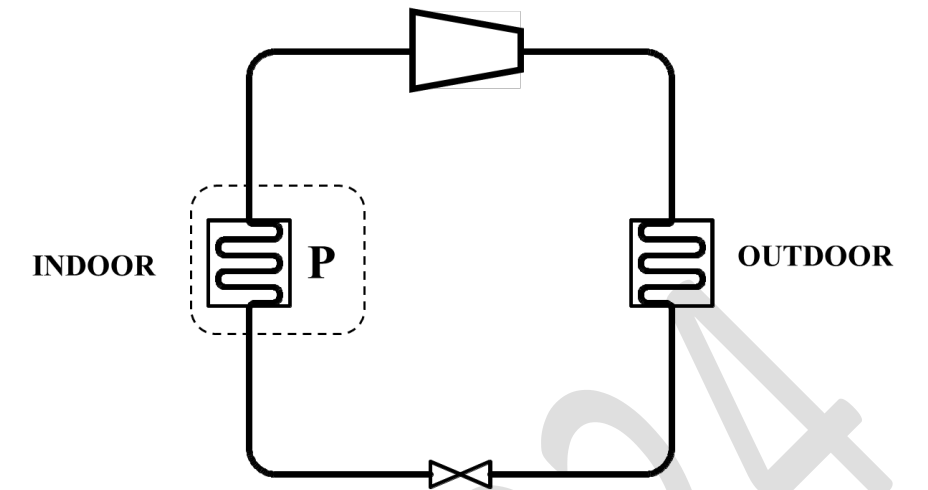
\includegraphics[width=0.5\columnwidth]{figs/12.jpg}
    \caption{Unitary Air-Conditioner}
    \label{fig:Img12}
    \end{figure}
    \begin{multicols}{4}
    \begin{enumerate}
        \item Condenser
        \item Evaporator
        \item Compressor
        \item Expansion valve
    \end{enumerate}
    \end{multicols}
    \hfill (GATE-AR 2024)

    \item Titan Integrity Campus, Bengaluru is designed by
    \begin{multicols}{2}
    \begin{enumerate}
        \item Christopher C. Benninger
        \item Sanjay Mohe
        \item Raj Rewal
        \item Anant Raje
    \end{enumerate}
    \end{multicols}
    \hfill (GATE-AR 2024)

    \item With reference to the Figure above, which of the following labelling is/are correct?
    \begin{figure}[h!]
    \centering
    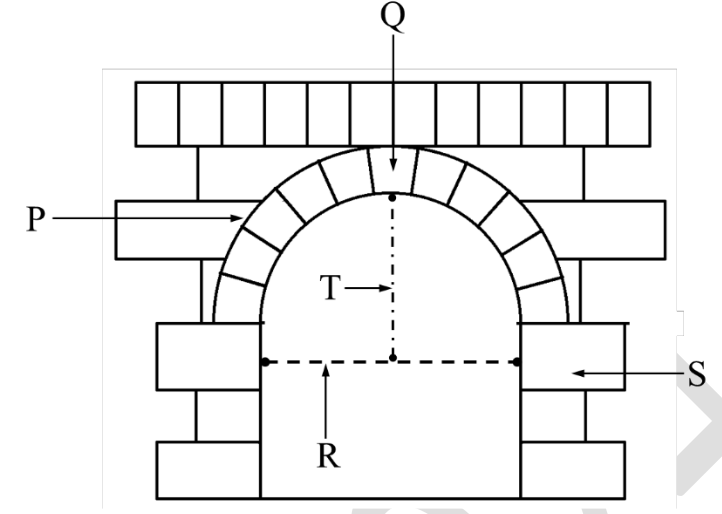
\includegraphics[width=0.3\columnwidth]{figs/13.jpg}
    \caption{}
    \label{fig:Img13}
    \end{figure}
    \begin{enumerate}
        \item P – Extrados, Q – Key , R – Span
        \item Q – Key, S – Abutment, T – Rise
        \item P – Abutment, R – Rise, T – Extrados
        \item Q – Key, S – Span, T – Extrados
    \end{enumerate}
    \hfill (GATE-AR 2024)

    \item Which of the following buildings has/have pendentives as a structural element?
    \begin{enumerate}
        \item St. Mark's Basilica, Venice, Italy
        \item Westminster Cathedral, London, UK
        \item Dilwara Temple, Mount Abu, India
        \item Hagia Irene Museum and Concert Hall, Istanbul
    \end{enumerate}
    \hfill (GATE-AR 2024)

    \item Polytetrafluroethylene (PTFE) coated fiberglass has been used as a roofing membrane in
    \begin{enumerate}
        \item Jawaharlal Nehru Stadium, New Delhi
        \item Eden Gardens Stadium, Kolkata
        \item Melbourne Cricket Ground Stadium, Melbourne
        \item Beijing National Stadium, Beijing
    \end{enumerate}
    \hfill (GATE-AR 2024)

    \item A non-stop express elevator directly connects the observatory level at 80\textsuperscript{th} floor of a tower with the podium at 2\textsuperscript{nd} floor level. The tower has a uniform floor-floor height of 4 m. The elevator attains a maximum speed of 8 m/s. Assume 2 m/s$^2$ as net vertical acceleration and net vertical deceleration (incorporating gravity). If the elevator starts from a state of rest from the podium, the time taken to reach the observatory, in seconds, is \rule{2cm}{0.4pt} (rounded off to one decimal place). \\
    \hfill (GATE-AR 2024)

    \item Match the elements in \textbf{Group—I} with the corresponding religious buildings in \textbf{Group—II}. \\
    \begin{tabular}{ l l }
    \textbf{Group—I} & \textbf{Group—II} \\
    (P) Bell capital & (1) Mosque \\
    (Q) Mehrab & (2) Hindu Temple \\
    (R) Gopuram & (3) Greek Temple \\
    (S) Pediment & (4) Romanesque Church \\
    & (5) Egyptian Temple \\
    \end{tabular}
    \begin{multicols}{2}
    \begin{enumerate}
        \item P—5, Q—1, R—2, S—3
        \item P—3, Q—1, R—5, S—4
        \item P—5, Q—4, R—3, S—2
        \item P—4, Q—1, R—2, S—3
    \end{enumerate}
    \end{multicols}
    \hfill (GATE-AR 2024)

    \item Match the museums in \textbf{Group—I} with their architects in \textbf{Group—II}. \\
    \begin{tabular}{ l l }
    \textbf{Group—I} & \textbf{Group—II} \\
    (P) Indira Gandhi Rashtriya & (1) Charles Correa \\
    Manav Sangrahalaya, Bhopal & \\
    (Q) Bihar Museum, Patna & (2) Ram Sharma \\
    (R) Gandhi Memorial Museum, & (3) Romi Khosla \\
    Ahmedabad & \\
    (S) Museum of Art and & (4) Soumitro Ghosh \& Nisha Mathew \\
    Photography, Bengaluru & \\
    & (5) Fumihiko Maki \\
    \end{tabular}
    \begin{multicols}{2}
    \begin{enumerate}
        \item P—4, Q—5, R—3, S—1
        \item P—4, Q—3, R—1, S—2
        \item P—2, Q—3, R—1, S—4
        \item P—2, Q—5, R—1, S—4
    \end{enumerate}
    \end{multicols}
    \hfill (GATE-AR 2024)

    \item Match the specially shaped bricks in \textbf{Group—I} with their corresponding nomenclature in \textbf{Group—II}.
    \textbf{Group-I}
    \begin{figure}[h!]
    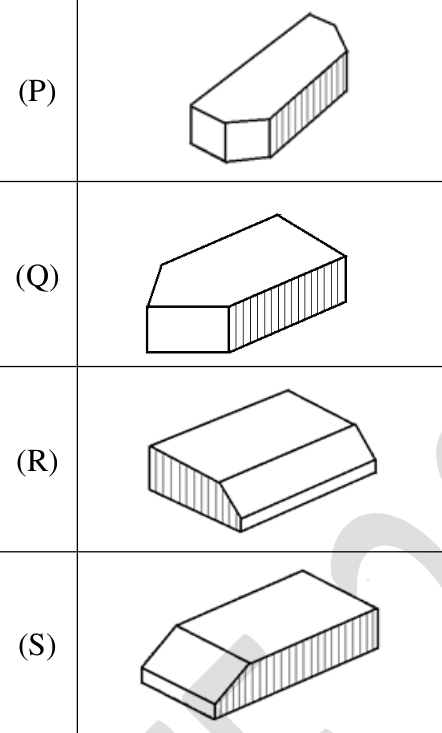
\includegraphics[width=0.2\columnwidth]{figs/14.jpg}
    \caption{Bricks}
    \label{fig:Img14}
    \end{figure} \\
    \textbf{Group—II} \\
    (1) Plinth Header \\
    (2) Bird's mouth \\
    (3) Squint \\
    (4) Double cant \\
    (5) Plinth stretcher
    \begin{multicols}{2}
    \begin{enumerate}
        \item P—4, Q—3, R—5, S—1
        \item P—3, Q—2, R—4, S—1
        \item P—4, Q—3, R—5, S—2
        \item P—4, Q—1, R—2, S—5
    \end{enumerate}
    \end{multicols}
    \hfill (GATE-AR 2024)

    \item Which of the following statements is/are correct?
    \begin{enumerate}
        \item The unit of Lighting Power Density is W/m$^2$.
        \item The unit of Lighting Power Density is cd/m$^2$.
        \item The unit of Sound Power is W.
        \item The unit of Energy Performance Index is kWh/m$^2$/year.
    \end{enumerate}
    \hfill (GATE-AR 2024)

    \item Which of the following statements is/are correct?
    \begin{enumerate}
        \item Kath-kuni construction comprises layers of stone and timber.
        \item Nalukettu houses have a courtyard.
        \item Ikra is a two-storeyed house with stone masonry and a flat-roof.
        \item Bhunga has a circular plan.
    \end{enumerate}
    \hfill (GATE-AR 2024)

\newpage

    \item A 5 m long Aluminium tie rod of cross-section 0.20 m $\times$ 0.04 m is subjected to a tensile force induced by its self-weight of 21.20 kg/m considering gravitational acceleration of 10 m/s$^2$. If tensile Young's modulus of Aluminium is 70,000 MPa, the maximum tensile strain in the rod is \rule{2cm}{0.4pt}$\times$10$^{-6}$ (rounded off to two decimal places). \\
    \begin{figure}[h!]
    \centering
    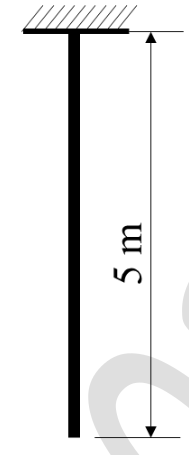
\includegraphics[width=0.2\columnwidth]{figs/15.jpg}
    \caption{Aluminium Tie Rod}
    \label{fig:Img15}
    \end{figure}
    \hfill (GATE-AR 2024)

    \item The following Figure shows the excavation plan of a two room structure, where the trench has a uniform width of 1.10 meters. If the cumulative centre line length of the trench is 41.10 meters and the required depth of concrete to be poured is 0.30 meters, the volume of concrete in foundation, in cubic meters, will be \rule{2cm}{0.4pt} (rounded off to two decimal places). \\
    \begin{figure}[h!]
    \centering
    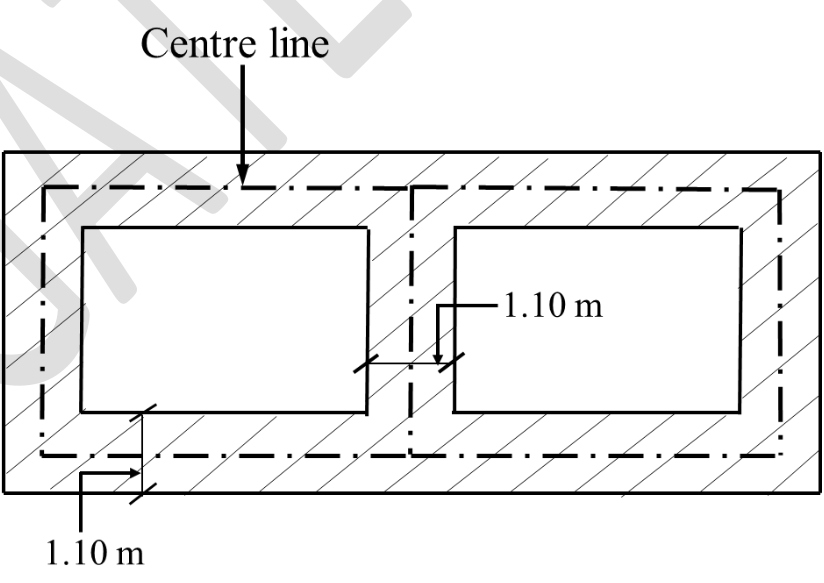
\includegraphics[width=0.5\columnwidth]{figs/16.jpg}
    \caption{Excavation Plan}
    \label{fig:Img16}
    \end{figure}
    \hfill (GATE-AR 2024)

\newpage

    \item The decay of sound in an enclosed lecture hall of volume 3500 m$^3$ is shown in the Figure below. The sound source is switched off at point \textbf{P}. Using the Reverberation Time ($RT_60$) obtained from the figure, the calculated total sound absorption of the hall, in Sabins, is \rule{2cm}{0.4pt} (rounded off to the nearest integer). \\
    \begin{figure}[h!]
    \centering
    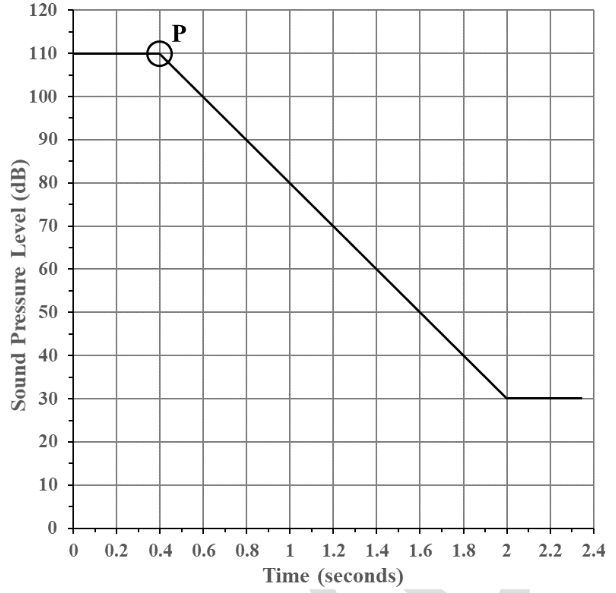
\includegraphics[width=0.5\columnwidth]{figs/17.jpg}
    \caption{Sound Pressure Level vs Time}
    \label{fig:Img17}
    \end{figure}
    \hfill (GATE-AR 2024)

    \item A 2 TR window air-conditioner of Energy Efficiency Ratio (EER) 3.1 is catering to a room of volume 40 m$^3$. The air-conditioner is operational for 600 hours during summer on cooling mode. The compressor is also operational for the complete duration. The total energy consumption of the air-conditioner during the above mentioned period, in kWh, is \rule{2cm}{0.4pt} (rounded off to nearest integer). \\
    \hfill (GATE-AR 2024)

\section*{PART B2: FOR Planning CANDIDATES ONLY}

    \item Which of the following aims is set under the SVAMITVA scheme of the Ministry of Panchayati Raj, Government of India?
    \begin{enumerate}
        \item Provide tap water connection to all households in rural areas.
        \item Provide 'right to work' to the rural people falling Below Poverty Line.
        \item Establish clear ownership of property in rural inhabited (Abadi) areas, by mapping of land parcels using improvised technology.
        \item Provide effective and efficient institutional platforms to enable the rural poor to increase their household income by means of sustainable livelihood enhancement.
    \end{enumerate}
    \hfill (GATE-AR 2024)

    \item Mass Rapid Transit System is a
    \begin{enumerate}
        \item Fixed Route and Fixed Schedule service.
        \item Fixed Route and Flexible Schedule service.
        \item Flexible Route and Fixed Schedule service.
        \item Flexible Route and Flexible Schedule service.
    \end{enumerate}
    \hfill (GATE-AR 2024)

    \item Which of the following initiatives of the Government of India is also known as the National Master Plan for Multi-modal Connectivity?
    \begin{multicols}{4}
    \begin{enumerate}
        \item PM Gati Shakti
        \item Bharatmala
        \item Parvatmala
        \item Sagarmala
    \end{enumerate}
    \end{multicols}
    \hfill (GATE-AR 2024)

    \item With reference to the Speed-Density diagram given below, which of the following statements is/are correct? \\
    \begin{figure}[h!]
    \centering
    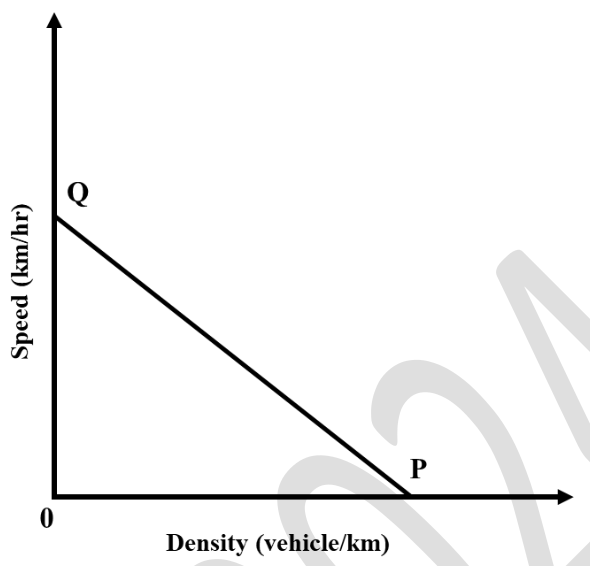
\includegraphics[width=0.5\columnwidth]{figs/18.jpg}
    \caption{Speed-Density Graph}
    \label{fig:Img18}
    \end{figure}
    \begin{enumerate}
        \item Point \textbf{P} represents Maximum Flow
        \item Point \textbf{P} represents Jam Density
        \item Point \textbf{Q} represents Space Mean Speed for Free Flow condition
        \item Point \textbf{Q} represents Time Mean Speed
    \end{enumerate}
    \hfill (GATE-AR 2024)

    \item Which of the following statements correctly represent(s) the Demographic dividend of a country?
    \begin{enumerate}
        \item Share of working age population is larger than dependent population.
        \item Share of working age population is lesser than dependent population.
        \item Demographic dividend demands more job creation.
        \item Demographic dividend can never lead to demographic disaster.
    \end{enumerate}
    \hfill (GATE-AR 2024)

    \item As per the URDPFI Guidelines 2015, choose the option(s) which indicate(s) the appropriate hierarchy of plans from higher to lower order.
    \begin{enumerate}
        \item Perspective Plan > Development Plan > Local Area Plan
        \item Development Plan > Special Purpose Plan > Annual Plan
        \item Local Area Plan > Development Plan > Annual Plan
        \item Special Purpose Plan > Perspective Plan > Local Area Plan
    \end{enumerate}
    \hfill (GATE-AR 2024)

    \item In 2021, a city survey report revealed a sex ratio of 930 with an estimated increase of 2.16\% over the next 20 years. In 2041, the total population of the city is projected to be 15,00,000. The estimated female population in the year 2041 will be \rule{2cm}{0.4pt} (in integer). \\
    \hfill (GATE-AR 2024)

    \item Match the terms in \textbf{Group—I} with their descriptions in \textbf{Group—II}. \\
    \begin{tabular}{ l l }
    \textbf{Group—I} & \textbf{Group—II} \\
    (P) Landfill site & (1) Development on previously developed site \\
    (Q) Greenfield development & (2) Land to dispose solid waste \\
    (R) Green Belt & (3) Development on previously undeveloped land \\
    (S) Brownfield development & (4) Policy to protect livestock \\
    & (5) A buffer to control urban development \\
    \end{tabular}
    \begin{multicols}{2}
    \begin{enumerate}
        \item P—2, Q—3, R—1, S—4
        \item P—3, Q—5, R—2, S—1
        \item P—2, Q—3, R—5, S—1
        \item P—3, Q—4, R—5, S—2
    \end{enumerate}
    \end{multicols}
    \hfill (GATE-AR 2024)

    \item Match the following illustrations in \textbf{Group—I} with their corresponding concepts in \textbf{Group—II}. \\
    \textbf{Group-I} \\
    \begin{figure}[h!]
    \centering
    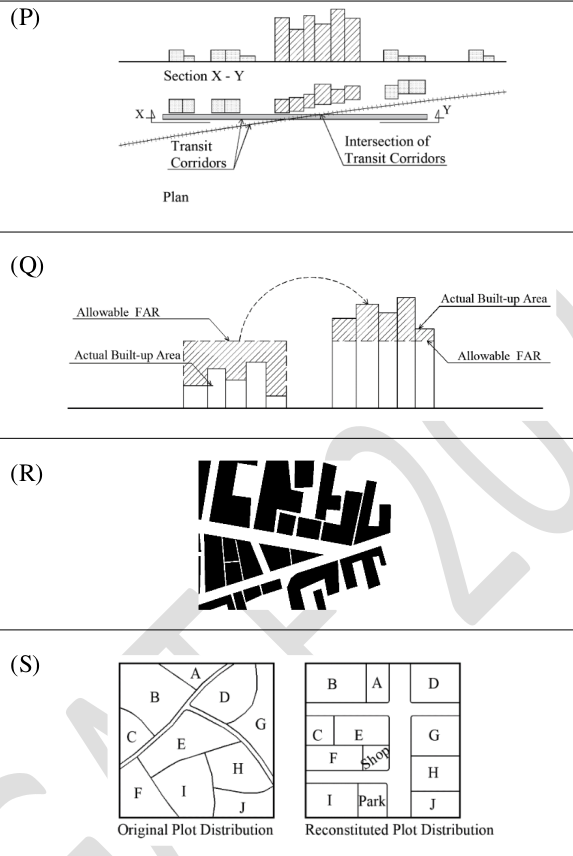
\includegraphics[width=0.5\columnwidth]{figs/19.jpg}
    \caption{}
    \label{fig:Img19}
    \end{figure} \\
    \textbf{Group—II} \\
    (1) Figure Ground Relationship \\
    (2) Town Planning Scheme (TPS) \\
    (3) Transit Oriented Development (TOD) \\
    (4) Transferable Development Rights (TDR) \\
    (5) Cul-de-Sac
    \begin{multicols}{2}
    \begin{enumerate}
        \item P—3, Q—4, R—1, S—2
        \item P—3, Q—5, R—2, S—4
        \item P—1, Q—3, R—4, S—2
        \item P—2, Q—4, R—1, S—5
    \end{enumerate}
    \end{multicols}
    \hfill (GATE-AR 2024)

    \item Match the following planning theories/concepts in \textbf{Group—I} with their corresponding proponents in \textbf{Group—II}. \\
    \begin{tabular}{ l l }
    \textbf{Group—I} & \textbf{Group—II} \\
    (P) Valley Section & (1) McGee and Gemburg \\
    (Q) Third Place Theory & (2) Oscar Newman \\
    (R) Defensible Space & (3) Ray Oldenberg \\
    (S) Desakota Model & (4) Patrick Geddes \\
    & (5) C. A. Doxiadis \\
    \end{tabular}
    \begin{multicols}{2}
    \begin{enumerate}
        \item P—4, Q—3, R—2, S—1
        \item P—4, Q—2, R—3, S—1
        \item P—1, Q—3, R—5, S—2
        \item P—2, Q—4, R—1, S—5
    \end{enumerate}
    \end{multicols}
    \hfill (GATE-AR 2024)

    \item Which of the following methods is/are used in traffic survey to measure the Running Speed and Journey Speed?
    \begin{multicols}{2}
    \begin{enumerate}
        \item Moving Observer Method
        \item Registration Number Method
        \item Elevated Observer Method
        \item Hardy Cross Method
    \end{enumerate}
    \end{multicols}
    \hfill (GATE-AR 2024)

    \item In the context of regional planning, which of the following terms represent(s) a region?
    \begin{multicols}{4}
    \begin{enumerate}
        \item Formal
        \item Functional
        \item Isometric
        \item Planning
    \end{enumerate}
    \end{multicols}
    \hfill (GATE-AR 2024)

    \item In a one-way single lane traffic stream, the observed average time headway is 2.5 seconds. The traffic flow of the above mentioned lane, in vehicle/hr, is \rule{2cm}{0.4pt} (in integer). \\
    \hfill (GATE-AR 2024)

    \item The demand of a EcoCity theme park is estimated as P = 1500 ${-}$ 7.5Q, where P (in Indian Rupees) is the price of a ticket for single entry, and Q (in integer) is the number of tickets sold per hour. The maximum revenue per hour along the demand curve, in Indian Rupees, is \rule{2cm}{0.4pt} (in integer). \\
    \hfill (GATE-AR 2024)

    \item Labour supply and urban growth are represented in X and Y axis of the Figure below. Curve OP represents the relationship between labour supply and urban growth. The ratios A:A' and B:B' are 1:1.2 and 3:1.2, respectively. If 6 units of labour is supplied in B, then the number of units of urban growth in B' will be \rule{2cm}{0.4pt} (rounded off to one decimal place). \\
    \begin{figure}[h!]
    \centering
    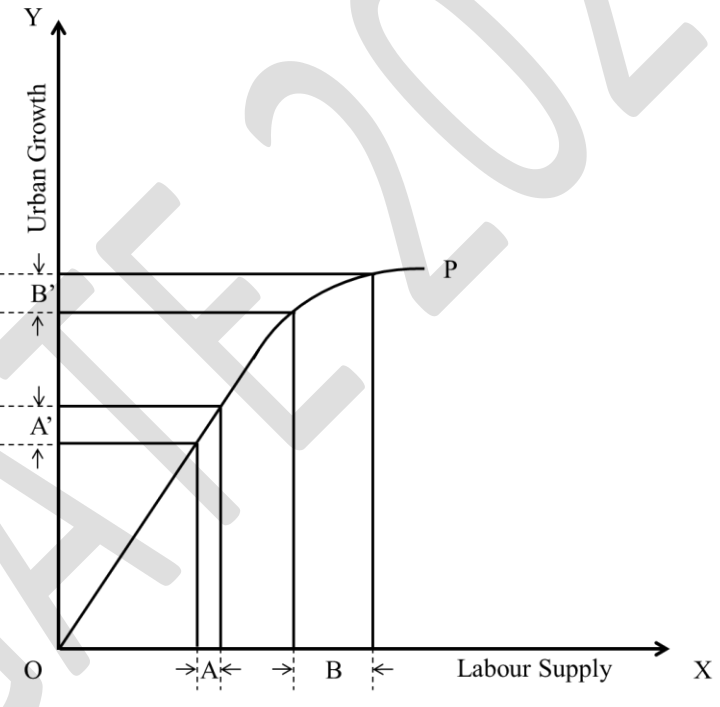
\includegraphics[width=0.4\columnwidth]{figs/20.jpg}
    \caption{Curve OP}
    \label{fig:Img20}
    \end{figure}
    \hfill (GATE-AR 2024)
    
\newpage

    \item A city with a present population of 1,75,000 is expecting an annual population growth rate of 0.85\%. In a traffic assessment study, the trip generation model has been developed as $Y = 142 + 0.675X$, where Y is the number of daily trips generated within the city and X is the population of the city. The number of daily trips to be generated within the city after 10 years is \rule{2cm}{0.4pt} (in integer). \\
    \hfill (GATE-AR 2024)

\end{enumerate}

\centering
\section*{END OF THE QUESTION PAPER}

\end{document}
